%%%%%%%%%%%%%%%%%%%%%%%%%%%%%%%%%%%%%%%%%
% 中文简体模板
% 版本:1.0 (2024.08.21)
% 修改者:ZJW
% 编译器:XeLaTeX
%%%%%%%%%%%%%%%%%%%%%%%%%%%%%%%%%%%%%%%%%

%----------------------------------------------------------------------------------------
%	封面与文档设置
%----------------------------------------------------------------------------------------
\documentclass[12pt, aspectratio=169]{beamer} 
%%%%%%%%%%%%%%%%%%%%%%%%%%%%%%%%%%%%%%%%%
% 中文简体模板
% 版本:1.0 (2024.08.21)
% 修改者:ZJW
% 编译器:XeLaTeX
%%%%%%%%%%%%%%%%%%%%%%%%%%%%%%%%%%%%%%%%%

%----------------------------------------------------------------------------------------
%	封面及全局配置
%----------------------------------------------------------------------------------------
\usepackage{fontspec} 
%----------------------------------------------------------------------------------------
%	中文字体 (选择其中1个)
% 
% 	AutoFakeBold=3.5: 粗体的深度
% 	AutoFakeSlant=0.2: 斜体的深度
% 	Path = fonts/: 字体的路径
%----------------------------------------------------------------------------------------
\usepackage{xeCJK}
% \setCJKmainfont[AutoFakeBold=3.5 , AutoFakeSlant=0.2, Path = fonts/]{cwTeX_圓體.ttf}
% \setCJKmainfont[AutoFakeBold=3.5 , AutoFakeSlant=0.2, Path = fonts/]{SIMHEI.ttf} % 黑体
% \setCJKmainfont[
%     Path=fonts/, % 字体文件所在路径
%     BoldFont=MSYHBD.ttc, % 粗体
%     ItalicFont=MSYH.ttc, % 斜体(微软雅黑不区分斜体,所以用常规字体代替)
%     SlantedFont=MSYH.ttc, % 斜体(如果需要,可以设置与常规字体一致)
%     BoldItalicFont=MSYHBD.ttc, % 粗斜体(如果需要,可以设置与粗体一致)
%     AutoFakeBold=3.5, % 自动加粗
%     AutoFakeSlant=0.2 % 自动倾斜
% ]{MSYH.ttc} % 微软雅黑
% \setCJKmainfont[AutoFakeBold=3.5 , AutoFakeSlant=0.2, Path = fonts/]{华文行楷.ttf} 
\setCJKmainfont[AutoFakeBold=3.5 , AutoFakeSlant=0.2, Path = fonts/]{SIMSUN.ttc} % 宋体
% \setCJKmainfont[AutoFakeBold=3.5 , AutoFakeSlant=0.2, Path = fonts/]{SIMKAI.TTF} % 楷体
\XeTeXlinebreaklocale "zh" % 這兩行用來調整中文自動換行
\XeTeXlinebreakskip = 0pt plus 1pt

%----------------------------------------------------------------------------------------
%	英文字体 (选择其中1个)
% 
%----------------------------------------------------------------------------------------
% \usefonttheme{serif} % 使用 serif 字體
\setmainfont[
    Path=fonts/,
    UprightFont=TIMES.TTF,
    BoldFont=TIMESBD.TTF,
    ItalicFont=TIMESI.TTF,
    BoldItalicFont=TIMESBI.TTF
]{Times New Roman} % Times New Roman

\usepackage{color} 
%% 自定义颜色
\definecolor{JLUPurple}{RGB}{102,8,116}
\definecolor{JLUGreen}{RGB}{0,166,82}
\definecolor{JLURed}{RGB}{157,41,51}
\definecolor{JLUBlue}{RGB}{0, 0, 128}

\usepackage{mathtools, amsmath, amsfonts, amsthm, latexsym} 
\usepackage{newtxtext,newtxmath}
\usepackage[justification=centering]{caption} 
\setbeamertemplate{caption}[numbered]
\captionsetup[figure]{font=small, labelfont=md}
\captionsetup[table]{font=small, labelfont=md}
\usepackage{graphicx}  
\usepackage{booktabs}
\usepackage{subfigure} 
\usepackage{multirow} 
\usepackage{array}
\usepackage{enumerate} 
\usepackage{tikz}
\usepackage{natbib}
\usepackage{comment}
\renewcommand{\figurename}{图} 
\renewcommand{\tablename}{表} 

%----------------------------------------------------------------------------------------
%	排版形式 (选择其中1个)
%----------------------------------------------------------------------------------------

\mode<presentation>{
% \usetheme{default} 
% \usetheme{AnnArbor}  
% \usetheme{Antibes}
% \usetheme{Bergen}
% \usetheme{Berkeley}
% \usetheme{Berlin}
% \usetheme{Boadilla}
% \usetheme{CambridgeUS}
% \usetheme{Copenhagen}
\usetheme{Darmstadt}
% \usetheme{Dresden}
%\usetheme{Frankfurt}
%\usetheme{Goettingen}
%\usetheme{Hannover}
%\usetheme{Ilmenau}
%\usetheme{JuanLesPins}
%\usetheme{Luebeck}
% \usetheme{Madrid}
%\usetheme{Malmoe}
%\usetheme{Marburg}
%\usetheme{Montpellier}
%\usetheme{PaloAlto}
%\usetheme{Pittsburgh}
%\usetheme{Rochester}
%\usetheme{Singapore}
%\usetheme{Szeged}
%\usetheme{Warsaw}

%----------------------------------------------------------------------------------------
%	外框形式 (选择其中1个)
%----------------------------------------------------------------------------------------

%\useoutertheme{default}
% \useoutertheme{infolines}
\useoutertheme{miniframes}
% \useoutertheme{smoothbars} 
%\useoutertheme{sidebar}
%\useoutertheme{split}
%\useoutertheme{shadow}
%\useoutertheme{tree}
%\useoutertheme{smoothtree}

%----------------------------------------------------------------------------------------
%	外框的个性化设置
%----------------------------------------------------------------------------------------
%\setbeamercolor{section in head/foot}{fg=black, bg=white} 
%\setbeamertemplate{mini frames}{}  
\setbeamerfont{headline}{size=\scriptsize}
\setbeamerfont{footline}{size=\scriptsize}
\setbeamertemplate{navigation symbols}{} 

%% 方案1:
%\setbeamertemplate{footline} 
%{\leavevmode%
%\hbox{%
%\begin{beamercolorbox}[wd=0.5\paperwidth,ht=3ex,dp=1ex,leftskip=3ex]%
%{author in head/foot}%
%{\scriptsize\textbf{\insertshortauthor}}%
%\end{beamercolorbox}%
%\begin{beamercolorbox}[wd=0.5\paperwidth,ht=3ex,dp=1ex,right]%
%{author in head/foot}%
%\scriptsize \textbf{{\insertframenumber{} / \inserttotalframenumber\hspace*{2ex}}} %頁碼控制選項
%\end{beamercolorbox}%
%}}

%% 方案2
%\setbeamertemplate{footline}[page number] 

%% 方案3:
%\setbeamertemplate{footline}[] 

%----------------------------------------------------------------------------------------
%	顏色主題 (选择其中1个)
%----------------------------------------------------------------------------------------

\usecolortheme{default}
%\usecolortheme{albatross}
%\usecolortheme{beaver}
%\usecolortheme{beetle}
%\usecolortheme{crane}
%\usecolortheme{dolphin}
%\usecolortheme{dove}
%\usecolortheme{fly}
%\usecolortheme{lily}
%\usecolortheme{orchid}
%\usecolortheme{rose}
%\usecolortheme{seagull}
%\usecolortheme{seahorse}
%\usecolortheme{whale}
%\usecolortheme{wolverine}

%----------------------------------------------------------------------------------------
%	顏色主題的个性化设置
%----------------------------------------------------------------------------------------
\setbeamercolor{structure}{fg=JLUPurple} 
%\setbeamercolor{title}{bg=green, fg=black} 
%\setbeamercolor{frametitle}{bg=green,fg=black} 
%\setbeamercolor{normal text}{fg=orange}
%\setbeamercolor{block title}{bg=blue,fg=yellow} 
%\setbeamercolor{block body}{bg=green,fg=red} 
\setbeamercolor{alerted text}{fg=red} 

%----------------------------------------------------------------------------------------
%	enumerate 及 item 的形狀
%----------------------------------------------------------------------------------------

\useinnertheme{rounded} 
%\useinnertheme{circles} 
%\useinnertheme{rectangles}
%\useinnertheme{inmargin} 

%----------------------------------------------------------------------------------------
%	个性化 item 的顏色
%----------------------------------------------------------------------------------------
%\setbeamercolor{item projected}{bg=red}

%----------------------------------------------------------------------------------------
%	个性化页面
%----------------------------------------------------------------------------------------
\setbeamersize{text margin left=0.8cm, text margin right=0.8cm}
\special{papersize=\the\paperwidth,\the\paperheight}
\providecommand{\tabularnewline}{\\}
}

%----------------------------------------------------------------------------------------
%	背景
%----------------------------------------------------------------------------------------
% \setbeamertemplate{background}{
\includegraphics[height=\paperheight]{Fig/Background.png}}
\usebackgroundtemplate{%
	\tikz[overlay, remember picture] 
	\node[opacity=0.3, below=-1.25cm, at=(current page.center)] 
	{
\includegraphics[scale = 0.14]{Fig/JLU_LOGO.png}}; 
	}
 

\begin{document}
\title[\LaTeX{}  Beamer 如何做?]{\Huge{\textbf{吉林大学\LaTeX{} Beamer 模板}}} 
\subtitle{各种功能的展示} 

% 作者
\author[甄继伟]{% 
甄继伟  \thanks{\small 吉林大学数学系} \and%
JiWei Zhen \thanks{\small JiLin University}
}

% 学校
\institute[JLU]{\normalsize 吉林大学 JiLin University} 

% 日期
\date[\today]{\today}

%----------------------------------------------------------------------------------------
%	封面页
%----------------------------------------------------------------------------------------

\begin{frame}
	\titlepage 
\end{frame}

%----------------------------------------------------------------------------------------
%	目录
%----------------------------------------------------------------------------------------

\begin{frame}{\textbf{目录}}
	\tableofcontents 
\end{frame}

\beamersetuncovermixins{\opaqueness<1->{45}}{\opaqueness<1->{95}} 

\section{文本处理}

%----------------------------------------------------------------------------------------

\linespread{1}  
\begin{frame}{\textbf{文本处理}}
\linespread{1.5} 

	文字演示
	
	\bigskip 
	 
	\pause 
	
	 \alert{Econometrics} is a \textbf{statistical} method used to \textit{estimate} the economic relationship,
	 test economic theories, and evaluate the effects of government or business policies.
	 
	 \pause
	
	\bigskip 

	\begin{quote}
		Pure mathematics is, in its way, the poetry of logical ideas.\\
		(纯粹数学,就其本质而言,就是逻辑思想的诗篇。)\\
		--- Albert Einstein (爱因斯坦)
	\end{quote}
	
\end{frame}

%----------------------------------------------------------------------------------------
\section{项目编号及数字编号}

\linespread{1} 
\begin{frame}[<+>]{\textbf{项目编号及数字编号序列编号}}
\linespread{1.5} 

	\begin{itemize}[]
		\item 这是封面 itemize 的 item
		\begin{enumerate}[] 
			\item 这是封面 enumerate 的 item
			\item 比较一下两者:
				\begin{enumerate}[1] 
					\item 封包 itemize 的 item 的明显特点是小一些
					\item 封包 enumerate 的 item 的明显特点是大一些
					\item 另外,可见文字越往内层会逐渐稍微缩小。
				\end{enumerate}
		\end{enumerate}
	\end{itemize}
	
\end{frame}

%----------------------------------------------------------------------------------------
\section{数学符号}
\linespread{1} 
\begin{frame}{\textbf{数学的区块文字}}
\linespread{1.5}

	\begin{block}{\textbf{定义}} 
		一个二次可微分的实数函数$f\left(x\right)$称为一个凸函数(convex function),
		若$f^{\,\prime\prime}\!\left(x\right)\ge0$对所有的$x$;
		同理若$f^{\,\prime\prime}\!\left(x\right)\le0$对所有的$x$,
		则称为凹函数(concave function)。
	\end{block}
	
	\begin{block}{\textbf{证明}} 
		若要在证明的方块后加入实心正方形,
		加上$\backslash$hfill\$$\backslash$blacksquare\$。
		\hfill$\blacksquare$
	\end{block}
	
\end{frame}

%----------------------------------------------------------------------------------------

\linespread{1} 
\begin{frame}{\textbf{数学的区块文字 (续)}}
\linespread{1.5} 

	\begin{alertblock}{\textbf{引理}}
		这里是一个引理的例子。
	\end{alertblock}
	\label{链接的文字} 
	
	\begin{example}
		可以发现3个环境指令的不同
		\begin{itemize}
			\item block(证明):与背景色一致
			\item alertblock(引理):是红色的
			\item example(例子):是绿色的
		\end{itemize}
	\end{example}
	
\end{frame}

%----------------------------------------------------------------------------------------

\linespread{1} 
\begin{frame}[<+>]{\textbf{数学方程式}}
\linespread{1.5} 
	\begin{align}\label{reg}
		\ln\left[\frac{Prob.\left(Y=b|X\right)}{Prob.\left(Y=0|X\right)}\right]
			=\beta_0+\sum_{j=1}^k \beta_{i,j}\,X_{i,j,b|Y=0}+\varepsilon_{i,b|Y=0}
	\end{align}

	\begin{align}\label{var}
		\left(n-1\right)\!S^{\,2} & =  \sum_{i=1}^{n}\left(x_{i}-\widebar{X}\right)^{2} 
			 =  \sum_{i=1}^{n}x_i^{\,2}-n\widebar{X}^{\,2} \notag \\
		\Rightarrow \sum_{i=1}^{n} x_i^{\,2} & =  \left(n-1\right)\!S^{\,2}+\underbrace{n \widebar{X}^{\,2}}_{\text{校正项}}
	\end{align}

\end{frame}


\section{图标制作}

%----------------------------------------------------------------------------------------
\subsection{图片}
\linespread{1}  
\begin{frame}{\textbf{插入图片}}
\linespread{1.5}
	
	\begin{figure}
		\centering % 置中
		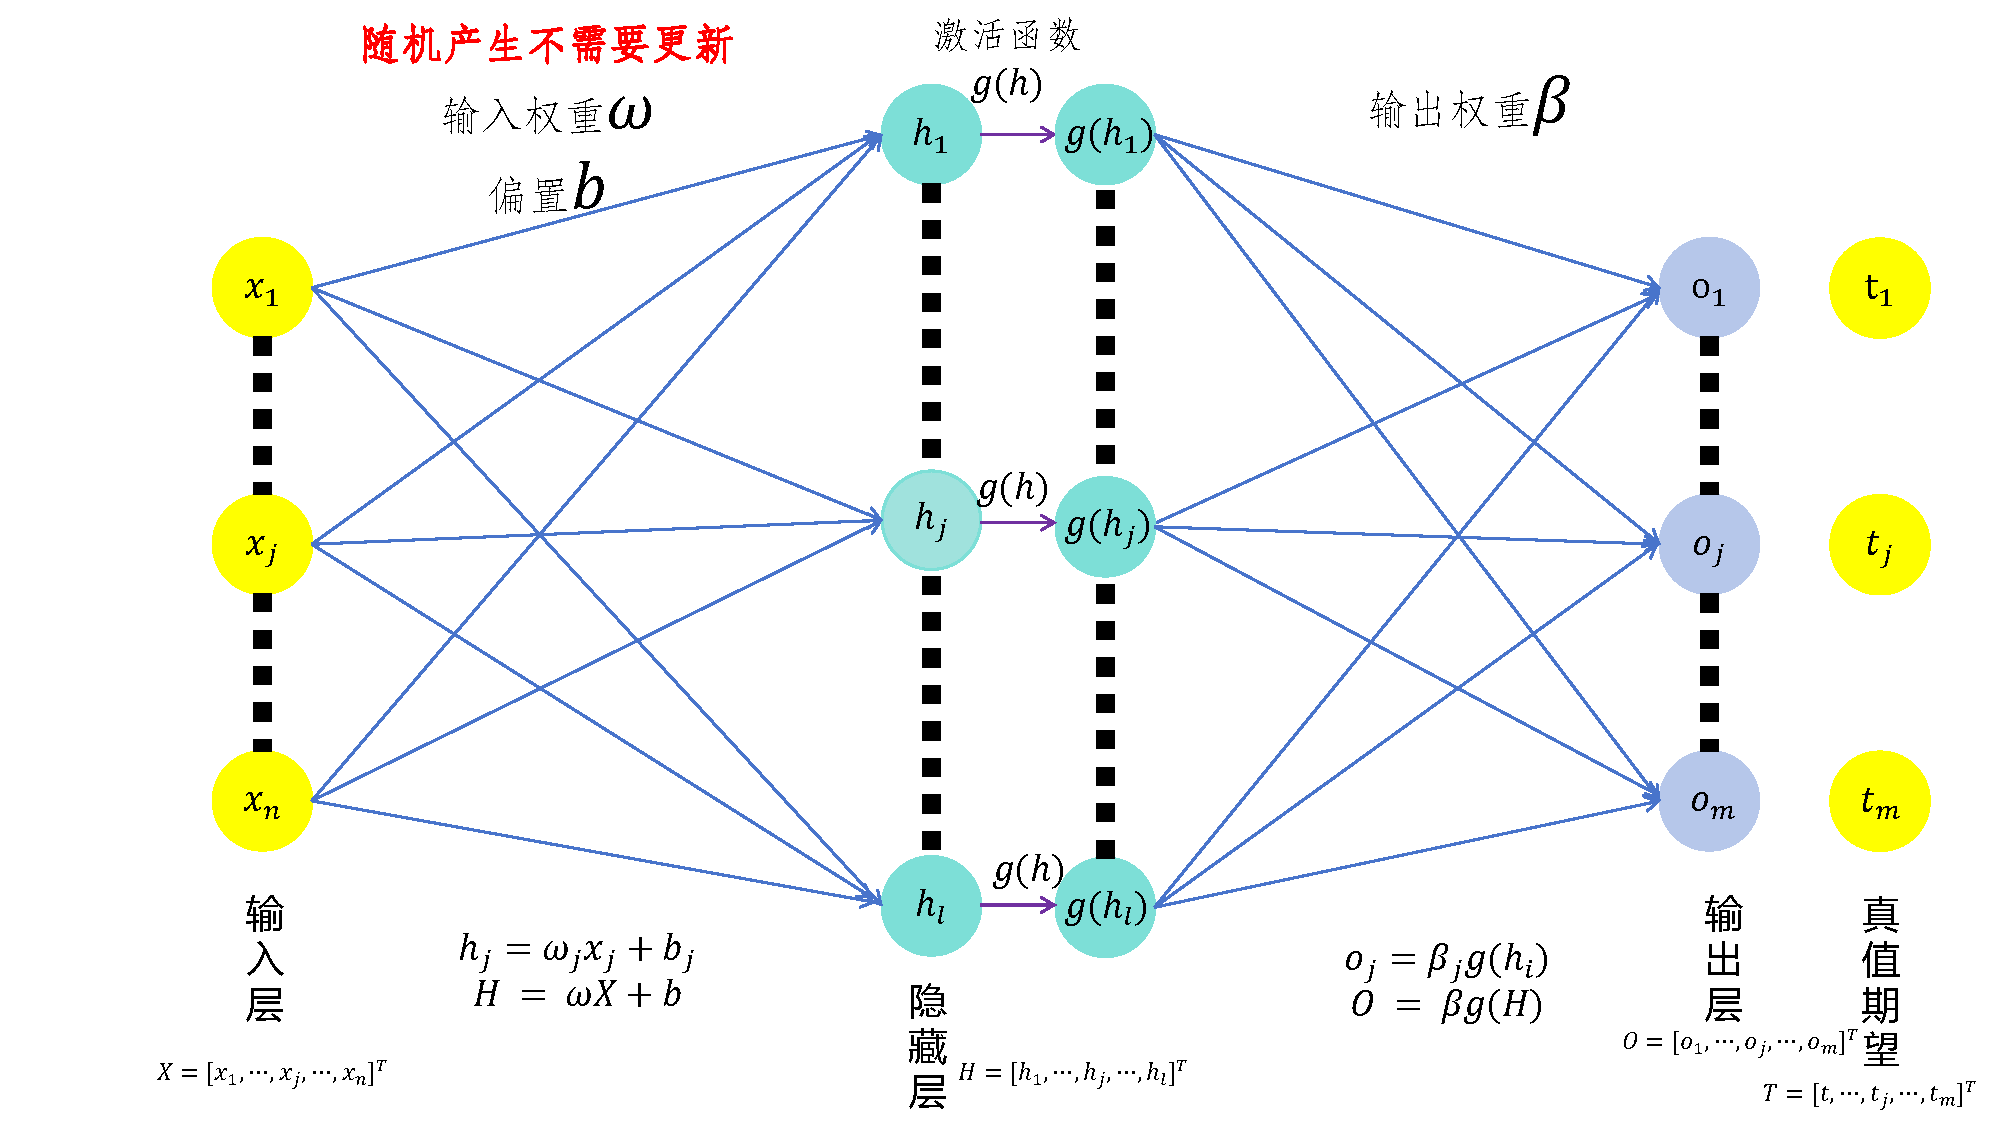
\includegraphics[scale=0.3]{Fig/单隐层前馈神经网络(SLFN).pdf}\\ % 插入图片
		\hspace{-9em}\scriptsize{图片来源:ZJW's BLOG} % 图片来源
		\vspace{-0.5em} % 缩减垂直距离
		\caption{单隐层前馈神经网络(SLFN)} % 图片名称
		\label{SLFN} % 图片标签
	\end{figure}
	
\end{frame}

%----------------------------------------------------------------------------------------
%	加入单页表格
%----------------------------------------------------------------------------------------
\subsection{表格}

\linespread{1}  
\begin{frame}{\textbf{插入表格}}
\linespread{1.5} 

	\begin{table}[htbp]
		\centering % 置中
		\caption{吉林大学本科统考数据汇总(2022/2023年度)} % 表名
		\extrarowheight=2pt % 額外增加每列的寬度
		\label{loan} % 建立表標籤
		\scalebox{0.9}{ % 將表縮小,不要縮小可以調成 1。
		\begin{tabular}{p{5cm} p{3cm}<{\centering} p{3cm}<{\raggedleft}} % 控制欄寬,及文字對齊方式。
			\toprule
			\midrule
 			& 2022年 & 2023年\\
			\midrule
			数学专业 & 56 & 58 \\
			计算机科学与技术 & // & 53 \\
			人工智能 & 6 & 6 \\
			软件工程 & 48 & 48 \\
			\midrule
			\bottomrule
		\end{tabular}
		}
		\par\smallskip
		\hspace{2em}\parbox{0.8\textwidth}{\scriptsize % 調整資料來源及表註的位置、字體大小及文字寬度。
		资料来源:\href{https://zsb.jlu.edu.cn/index/examscores.html}{本科统考数据汇总}。\par
		注:\parbox[t]{0.6\textwidth}{\scriptsize % 記得稍微小於前兩行的 \textwidth
		可在这里添加备注。
		}
		}
	\end{table}
	
\end{frame}


%----------------------------------------------------------------------------------------

\linespread{1} 
\begin{frame}{\textbf{插入表格 (续)}}
\linespread{1.5} 

	\begin{table}[htbp]
		\centering 
		\caption{近五年五大最佳行业} 
		\extrarowheight=2pt 
		\label{CareerCast} 
		\scalebox{0.8}{ 
		\begin{tabular}{@{}crrrr@{}} 
			\toprule
			\midrule
			 排名 & 2021 &  2019 & 2018 & 2017\\
			\midrule
			1 & \textbf{IT互联网} & \textbf{IT互联网}  &  金融 & \textbf{IT互联网} \\
			2 & \textbf{电子半导体} & 金融 & \textbf{IT互联网}  & 金融 \\
			3 & 服务行业 & \textbf{电子半导体}  & 服务行业 & \textbf{电子半导体}\\
			4 & 金融 & 医疗  & \textbf{新能源} & 房地产 \\
			5 & \textbf{机械制造} & 服务行业 & \textbf{新能源} & 服务行业 \\
			\midrule
			\bottomrule
		\end{tabular}
		}
		\par\smallskip
		\hspace{0.5em}\parbox{0.6\textwidth}{\scriptsize
		资料来源:ChatGPT, 取自:\url{https://chat.openai.com}。\par
		注:\parbox[t]{0.5\textwidth}{\scriptsize
			1、chatGPT生成不确定一定正确的答案。\\
		 	2、粗体为理工科 (STEM) 相关行业。
		}
		}
	\end{table}

\end{frame}

%----------------------------------------------------------------------------------------
\section{两栏图文}
\linespread{1}  
\begin{frame}{\textbf{两栏图文 (或多栏)}}
\linespread{1.5} 

	\begin{columns}[c]
		\column{0.67\textwidth} 
			\begin{enumerate}[]
				\item 我们在内文中要提及前面的图、表或方程式时,应该这样引注:
				\begin{enumerate}[]
					\item 「图 $\backslash$ref\{label 內的名字\}」,
						即可出现图 \ref{SLFN} 和图 \ref{LaTeX}。
					\item 「表 $\backslash$ref\{label 內的名字\}」,
						即可出现表 \ref{loan} 和表 \ref{CareerCast}。
					\item 「式 ($\backslash$ref\{label 內的名字\})」,
						即可出现式 (\ref{reg}) 和式 (\ref{var})。
				\end{enumerate}
				\item 引注的好处是简报有所更动时,不用一直手动调整编号。
			\end{enumerate}

		\column{0.33\textwidth}  
			\begin{figure}
				
\includegraphics[scale=0.045]{Fig/LaTeX.png}\\
				\scriptsize{图片来源:
				\href{https://en.wikipedia.org/wiki/LaTeX}{維基百科}。}\\
				\caption{\LaTeX}
				\label{LaTeX} 
			\end{figure}
	\end{columns}
\end{frame}


%----------------------------------------------------------------------------------------
%	其他
%----------------------------------------------------------------------------------------

\begin{frame}

	建立无标题页面,并展示超链接按钮。
	
	\bigskip
	
	\hyperlink{链接的文字}{\beamergotobutton{点击跳转链接}}
	
\end{frame}

%----------------------------------------------------------------------------------------
\section{参考资料}
\linespread{1} 
\begin{frame}{\textbf{引用参考资料的方法}}
\linespread{1.5}

	引用参考资料的方法:
	
	\begin{enumerate}[1]
		\item 将文献作者当作主语时使用时:\textbackslash citet\{给定的标签\}。
		\item 行文末端作为补充说明时:\textbackslash citep\{给定的标签\}。
	\end{enumerate}
	
	\bigskip
	
	以文本为例:
	
	\begin{enumerate}[1]
		\item \citet{Polynomial_Galerkin} 与 \citet{脉冲微分方程COVID-19}
		\item \citep{Polynomial_Galerkin} 与 \citep{脉冲微分方程COVID-19}
	\end{enumerate}
	
\end{frame}

%----------------------------------------------------------------------------------------

\linespread{1} 
\begin{frame}{\textbf{参考资料}}
\linespread{1.5} 

\footnotesize

\begin{thebibliography}{99} 

	\bibitem[JJW (2019)]{Polynomial_Galerkin}
		JJW (2019). 
		\newblock Polynomial preserving recovery for a class of weak Galerkin finite element methods, 
		\newblock \emph{Journal of Computational and Applied Mathematics}, 2019(362), 528-539. 

	\bibitem[贾继伟 (2019)]{脉冲微分方程COVID-19} 
		贾继伟 (2019)。 
		\newblock 基于脉冲微分方程的COVID-19境外输入型病例对我国疫情防控影响的分析:2021年,
		\newblock \emph{中国科学·数学},51(4), 659。
		
\end{thebibliography}

\end{frame}

%----------------------------------------------------------------------------------------
\section*{结束页}
\begin{frame}[plain] 

	\begin{center}
		{\Huge \textbf{谢谢观看!}}
		
		\bigskip\bigskip 
		
		{\LARGE \textbf{欢迎提问!}}
	\end{center}
	
\end{frame}

%----------------------------------------------------------------------------------------

\end{document} 
